\section{Introduction}

The cloud is changing how users interact with data. This is true for
legacy applications that are migrating on-site data to cloud
storage, and for emerging applications that are augmenting
cloud storage and dataset repositories with edge caches. In both cases,
leveraging multiple cloud storage systems, edge caches, and dataset
repositories allows applications to harness their already-deployed infrastructure,
instantly gaining a global footprint.  However, doing so introduces
several storage design challenges relating to functional requirements,
data consistency, access control, and fault tolerance. This paper
describes \Syndicate, a wide-area storage system that addresses them 
in a coherent manner.

\begin{figure}[h!]
\centering
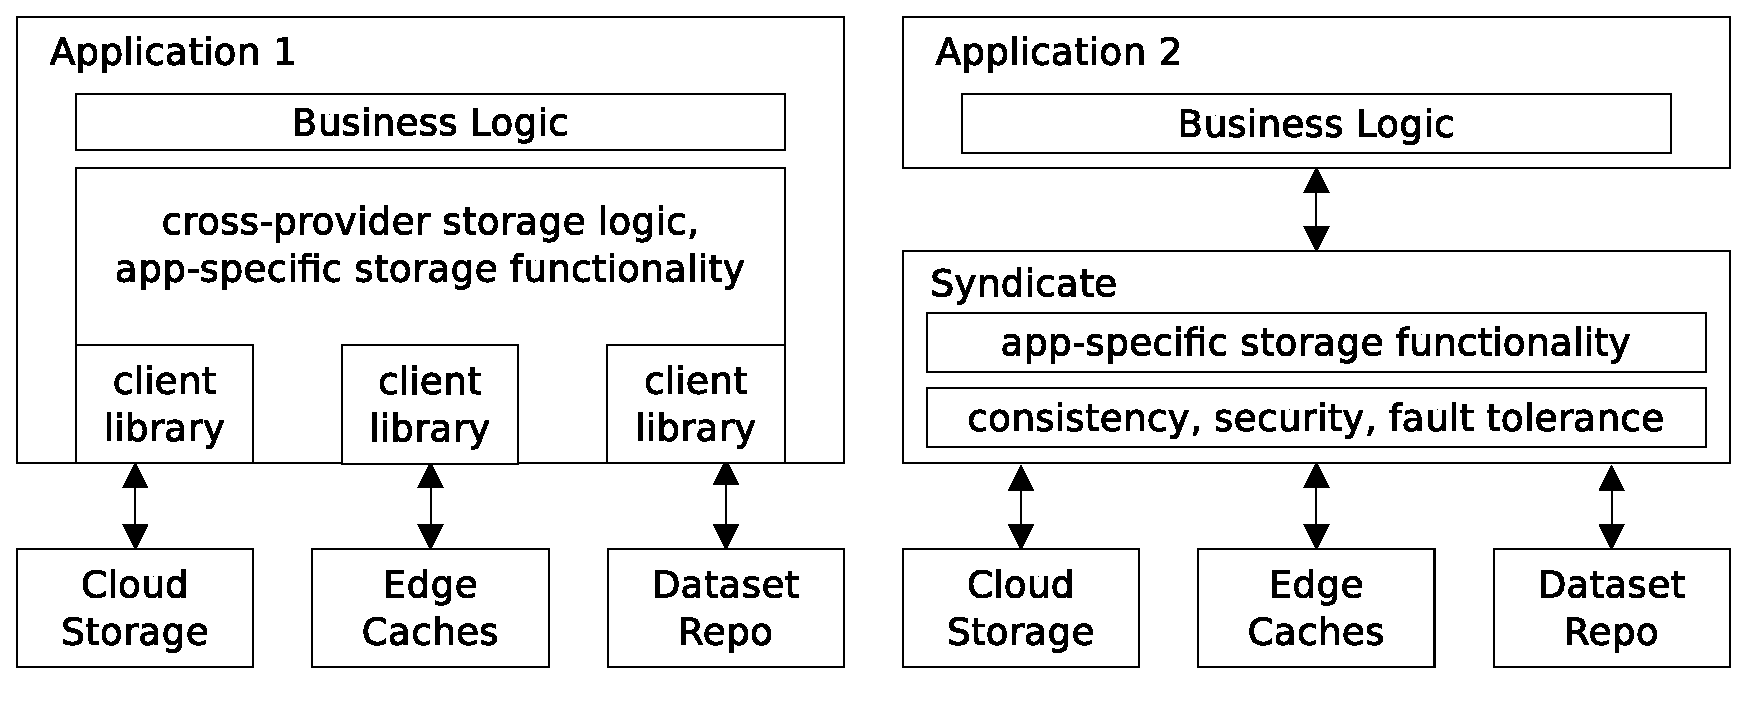
\includegraphics[width=0.47\textwidth]{figures/overview}
\caption{\it Application design with and without Syndicate.}
\label{fig:overview}
\end{figure}

Each type of component system offers well-understood
{\it functional} benefits.  Cloud storage offers an ``always-on''
repository for hosting a scalable amount of data, while keeping it
consistent and enforcing access controls.
Dataset repositories host and curate a scalable amount of read-only data on 
behalf of many applications.  CDNs, caching Web proxies, and HTTP object caches (``edge
caches'') help under-provisioned origin servers scale up the
volume of requests they can handle.
In all cases, instances of these systems ({\it providers}) make their 
functional benefits available through instance-specific APIs.

In contrast, the providers' infrastructure
offers two key \textit{utility} benefits transparently
---data durability and access locality.
Cloud storage and dataset providers improve durability by
replicating data to geographically distributed
datacenters, and edge caching providers improve locality by
placing temporary copies of data at sites closer to readers than the
origin servers (lowering latency and increasing bandwidth).

Unlike functional benefits, utility benefits can be aggregated.
Leveraging multiple providers yields more utility than leveraging any single
one, and improvements to one 
provider improve overall utility.
However, doing so is non-trivial because each provider
has a different API, with different functional semantics.  The developer
must design the application around this, thereby coupling its storage logic 
to provider implementations (Figure~\ref{fig:overview}, left).

Our key insight is that this coupling can be avoided by leveraging providers not for 
their functional benefits, but for the utility they offer---cloud
storage and dataset providers offer durability, and edge caching providers offer
locality.  While this strategy ultimately makes the developers responsible for storage functionality, doing so lets them
implement exactly the functionality they need while aggregating provider utility.
\Syndicate\ helps them implement and deploy this functionality at scale, while
minimizing provider coupling and addressing common storage concerns
on their behalf (Figure~\ref{fig:overview}, right).

The key contribution of \Syndicate\ is wide-area software-defined storage
service that runs on top of unmodified providers.  It provides an
extensible interface for implementing domain-specific storage
functionality in a provider-agnostic way, while addressing common cross-provider 
consistency, security, and fault-tolerance requirements automatically.
Using \Syndicate\ lets developers create a storage service for their applications 
that has the aggregate utility of multiple underlying providers, but without having to 
build and deploy a whole storage service from the ground up.
That is, \Syndicate\ creates virtual cloud storage through provider composition.
